\section{Technosignature Searches at Low Frequencies} \label{sec:method-technosignature-searches}

The first year of the project primarily entailed the publication \citep{johnson_simultaneous_2023} of results from the first search for technosignatues at low frequency using Irish and Swedish LOw Frequency ARay \citep[I-LOFAR;][] {van_haarlem_lofar_2013}. When carrying out this technosignature search the two main goals were to constrain the prevalance of intelligent civilizations in the Milky Way at an unexplored frequency and use the collected data to search for other exotic transients such as Fast Radio Bursts (FRBs), pulsars, magnetospheres and M-dwarf emission \citep{sheikh_nine_2020}. The following sections will detail the means and methods on how technosignature search is carried out.

\subsection{LOFAR}

LOFAR, a pioneering low-frequency aperture array telescope, spans hundreds of kilometers across Europe and serves as a pathfinder to the Square Kilometer Array (SKA). The array consists of a core station with outrigger stations situated in the Netherlands and additional international stations spanning multiple countries, such as Germany, France, Sweden, Ireland, Latvia, Poland, and the United Kingdom. Additionally, stations are currently in the process of being constructed in Italy and Bulgaria. The LOFAR array operates using two types of antenna, the Low Band Antenna (LBA) and the High Band Antenna (HBA), operating at $10–90$~MHz and $100–250$~MHz respectively\footnote{LBA: $\lambda \sim30 - 3$~m; HBA: $\lambda \sim3 - 1$~m}. In this study, the HBAs at the Irish and Swedish LOFAR station are used to carry out observations non interferometrically. The field of view (FoV) of an international LOFAR station is rather large; at full width at half maximum, it is 5.3, 3.4, and 2.3 deg$^2$ at frequencies of 120, 150, and 180 MHz, respectively \citep{van_haarlem_lofar_2013}. The station is capable of resolution of 3.3 and 0.2 arcsecond at the bottom and the top of the bad respectively when the entire array is in use making it one of the most sensitive telescopes in the world.

\subsection{Target Selection}

% Observation campaigns for this survey were carried out through the Summers of 2021 and 2022. Targets were selected for the survey based on exoplanet candidates from NASA's Transiting Exoplanet Survey Satellite \citep[TESS;][]{TESS2015}. In modern technosignature survey's the choice of exoplanet's surveyed is indifferent to characterstics of exoplanet and host star. This decision is due to the limited knowledge of ideal life harbouring conditions a planet must have. Instead the survey opts for sensitivity. Thus, targets were selected based on their distance ($\leq 1$ kpc) and altitude during time of observation. In total 44 TESS targets were observed \citep[see Table 2][]{johnson_simultaneous_2023}.

A significant fraction of radio emission from Earth is emitted in the direction of the ecliptic plane. For example, powerful planetary radars are used to explore Solar System objects \citep{Siemion_KEPLER_ApJ}, and high-powered transmitters are used to communicate with Solar System probes \citep{Enriquez2017ApJ}. It is conceivable then that such leakage radiation may also be emanating from other worlds, preferentially in their planetary orbital planes. This is why we chose TESS targets, as these are the closest transiting exoplanet systems known \citep{Kepler_Mission_Design_2010,TESS2015}. Observing these sources with the LOFAR HBAs enables robust constraints on any associated artificial low-frequency radio emission

\subsection{Expanding the Cosmic Haystack}

Searching for technosignatures is akin to searching for a needle is a cosmic sized haystack thus it is important to extend area of the haystack as much as possible. The beam of a LOFAR station has an expansive coverage enabling observation of a substantial number of stars in the field of view. The significance of these in-field stars has been highlighted by \cite{Bart-Wlodarczyk-Sroka}. Consequently, during our observations targeting 44 sources from the TESS catalog, we encountered a significant number of in-field stars within our field of view. \ 
To determine the list of targets within this field of view, the \textit{Gaia} catalog is utilized. Some previous major SETI surveys focused their searches toward Sun-like stars \citep{Tarter:1996jf}. However, because our understanding of the origin of life is limited, it makes sense to allow for the possibility of life arising on a planet that is neither Earth-like nor around stars that are Sun-like. Similarly, planets not necessarily located in the habitable zone should be considered. This is typically characterized as the orbital range wherein liquid water could exist \citep{Kasting1993}, as inferred from planetary equilibrium temperatures often ignoring the unknown albedo of the exoplanets. Any sensitive radio SETI survey seeking to maximize the chance of detecting weak radio signals should, insofar as possible, expand its search to encompass nearby stars of a broad range of spectral types and with exoplanets of all sizes and distances from their parent star. Thus, calculations were conducted to determine the number of Gaia stars with a mean distance of 1215 pc, with an accuracy in their distances of at least 20\%. This study used Gaia's third data release \cite[GDR3;][]{GaiaDR3,astroquery}. When analyzing GDR3, two filters were applied to the survey volume and sensitivity accuracy of the in-beam target values. First, a constraint on the R.A. and decl. errors was implemented. If a Gaia source was found to be in the beam but had an error magnitude greater than the FWHM, it was removed from the source pool. \Cref{Gaia:filter1} states the first condition of filtering:

\begin{equation}
    \theta_{\text{sep}} + \sqrt{\Delta \text{RA}^2 + \Delta \text{Dec}^2} \leq \frac{\text{FWHM}}{2}
    \label{Gaia:filter1}
\end{equation}

As the sensitivity of the survey is calculated based on a source's distance, a second filter is implemented to remove sources that have large errors. By taking the difference $(\Delta \sigma_G)$ in the upper and lower confidence levels of GSP-Photometry, we obtain a percentage error on distance. All sources with a $d_{M_G}$ error of 20\% or greater are filtered out of the source list. \Cref{Gaia:filter2} states the second condition of filtering:

\begin{equation}
    \frac{\Delta \sigma_G}{\sigma_G} \leq 20\%
    \label{Gaia:filter2}
\end{equation}

A total of 1,631,152 stars form this list, making it one of the largest samples of stars ever surveyed for SETI purposes.

\subsection{Carrying out a Dual-Site Survey}

% Following the selection of targets the survey is carried out using a custom pipeline. The pipeline developed for carrying out this survey is detailed in \cref{fig:SETI-pipeline}. Narrowband technosignatures have a width of a couple of Hz thus high frequncy resolution is required. As similarly discussed in \cref{sec:method-observation-data} the raw voltages need to be dignitized using a suite of software. In this case \texttt{GUPPI RAW} and \texttt{RAWSPEC}

\begin{figure}
    \centering
    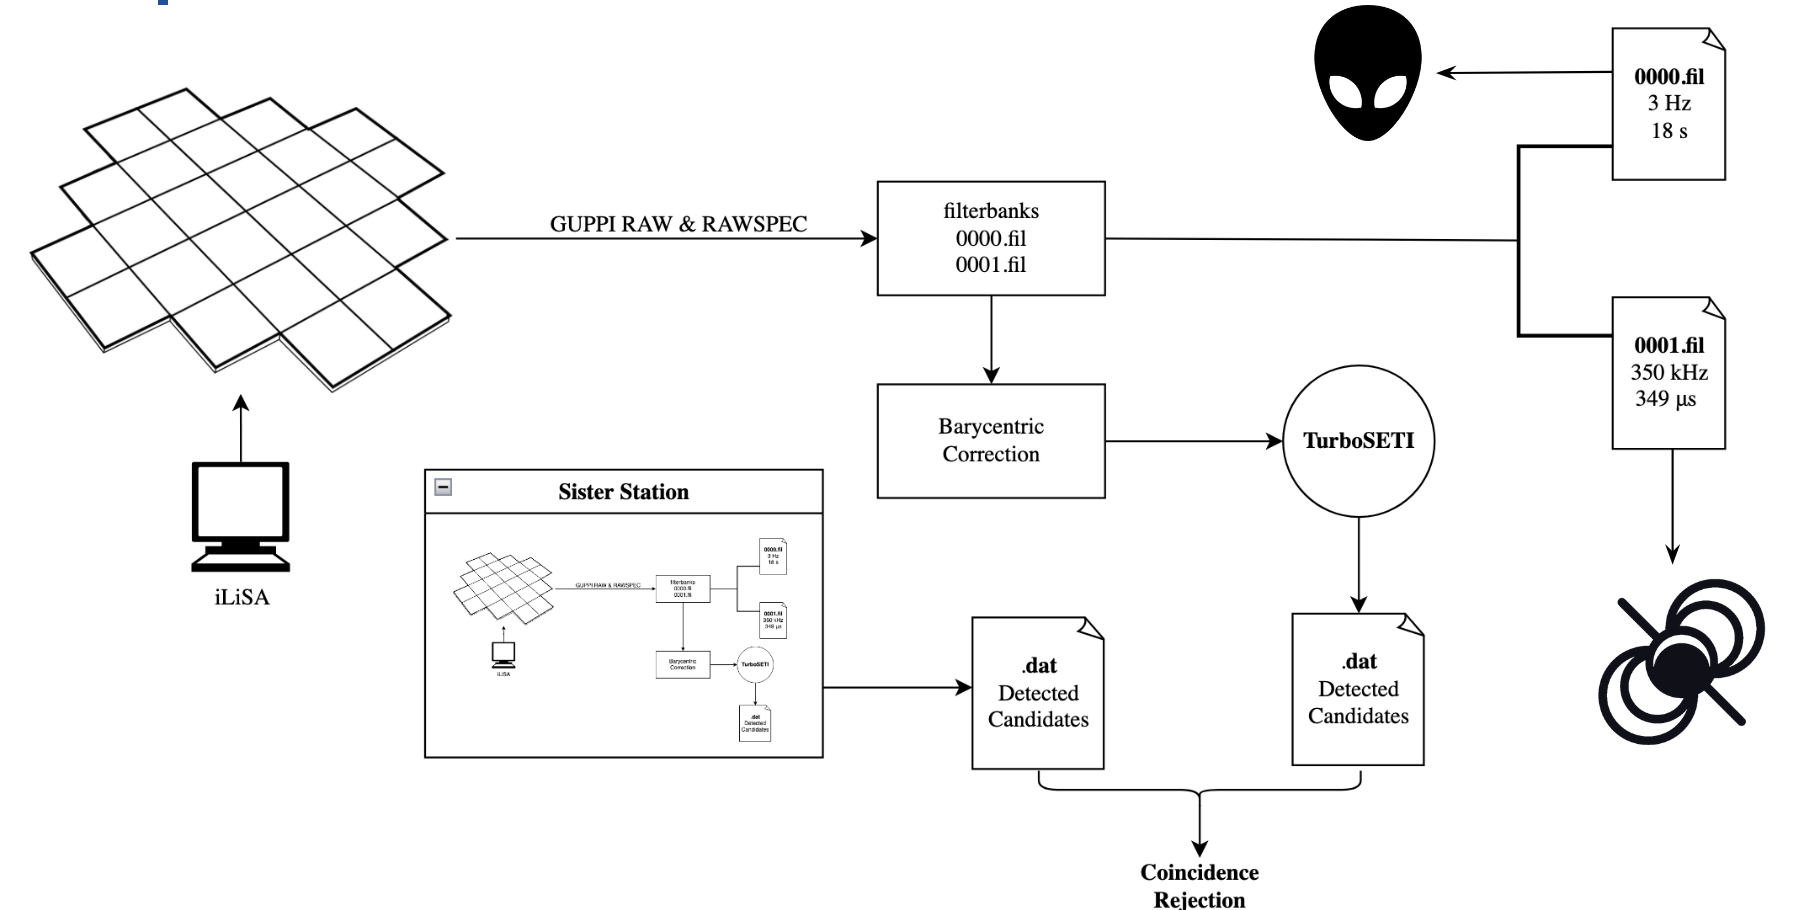
\includegraphics[width = 0.9\textwidth]{figs/SETI-pipeline.png}
    \caption{Outline of the SETI pipeline developed and deployed on Breakthrough Listen nodes at both LOFAR stations.}
    \label{fig:SETI-pipeline}
\end{figure}

Typically, international LOFAR stations operate as standalone telescopes $2-3$ days per week, i.e. they do not operate as part of the International LOFAR Telescope's Europe-wide array. This project was undertaken during this standalone time. For this purpose the \emph{international LOFAR in Stand-Alone mode} (\texttt{iLiSA}) package\footnote{\url{https://github.com/2baOrNot2ba/iLiSA/releases/tag/v6.1}} is used to control both telescopes simultaneously. \texttt{iLiSA} provides a high-level operational control of multiple LOFAR stations, including scheduling, processing pipeline dispatching and metadata aggregation. For the observations in this study, an operator-produced list of targets that were close\footnote{In practice as Birr and Onsala are separated by $\sim20\deg$ of longitude, the optimum scheduling is to observe $\sim 40$~min$-T_{\rm obs}/2$ `late' at Onsala and $40$~min$+T_{\rm obs}/2$ `early' at Birr.} to the local meridian was fed into \texttt{iLiSA} at each epoch. Towards each target, one beam per station was formed using \texttt{iLiSA}, and each beam was formed with $412$ HBA sub-bands (corresponding to a bandwidth of $80.46875$~MHz). The scan time on each target was $15$~min, and the whole scheduling block was a few hours per epoch. \ 
Data was preproccessed\footnote{For detailed explanation of the preprocessing and preperation see \cite{2019_Lebofsky}} and prepared using the \texttt{udpPacketManager} package \citep{David_JOSS}. Which resulted in two sets of filterbanks for each observation, each with different frequency and time resolutions. The first set of filterbanks had a frequency resolution of $2.98$~Hz and a temporal resolution of $0.67$~s. The second set of filterbanks had a frequency resolution of $350$~kHz and a temporal resolution of $349~\upmu\text{s}$. The first set of filterbanks was used for the search for narrowband technosignatures, and the second set was used for the search for broadband transients. A broad overview of the pipeline employed is shown in \cref{fig:SETI-pipeline}. \

\subsection{Narrowband Search Results}

Using \texttt{turboSETI}, a Doppler-drift search was carried out on the observed candidates at both stations. This resulted in the list of “hits” collected, where hits are defined as a narrowband signal detected above the given threshold, S/N = 10. The distribution of narrowband signals detected at both stations is shown in \cref{fig:hits-histogram}. A large percentage of hits are seen at both sites in the 120-140 MHz range. This falls within the range of expected RFI leakage seen from neighboring airports\footnote{Shannon \& Goteborg Landvetter.}. \ 
Using a drift-rate search of $\pm 4 \ \text{Hz/s}$ for this study covers a fraction of the possible drift rates of transmitters from exotic objects that can be detected as outlined by \cite{Sheikh_2019}. \cite{LiNarrowBand} shows that 4~Hz/s is comprehensive in relative to the expected distribution of exoplanet drift rates. The omission of a search outside this parameter space is due to its computationally intense nature of searching for narrow-band signals across a sizeable drift-rate range. However, in doing this, the parameter space searched for extra terrestrial intelligent (ETI) signal has been drastically reduced. Continual development of search algorithms like \verb|turboSETI| is progressing to make larger drift-rates searches a more computationally feasible. \
Upon first inspection of \Cref{fig:hits-histogram} it appears that the results at both stations are somewhat similar. However, upon performing a Kolmogorov-Smirnov (KS) test for each set of results for drift-rate, SN and frequency of detected hits the highest $p$-value returned was on the order of $10^{-11}$ indicating that the RFI environments at each of the stations are significantly different. \ 
In the case of this study, a singular beam observes a single target for 15 minutes at both stations and observations are converted to barycentric reference frame. Narrow-band searches are then performed at both sites, and the results of both searches are compared.

In our analysis, a signal is classified as a mutual extraterrestrial hit only if two conditions are met: \textit{a)} the signals are within a frequency range of $\pm 4 \ \text{Hz}$ of each other in the barycentric reference frame, and \textit{b)} their drift rates are within $\pm 0.2 \ \text{Hz/s}$ of each other after barycentric drift corrections. In the topocentric frame, a detected narrowband signal at 160 MHz that is simultaneously present at both stations. However, when converting to the barycentric reference frame, the signal appears to be seen at different frequencies with opposite signs due to the different line-of-sight velocities towards the target with both signals differing by 300 kHz. As a result, this narrowband signal is rejected as a genuine sky-bound signal.

\begin{figure} %[h!]
    \centering
    \subfloat[\centering]{{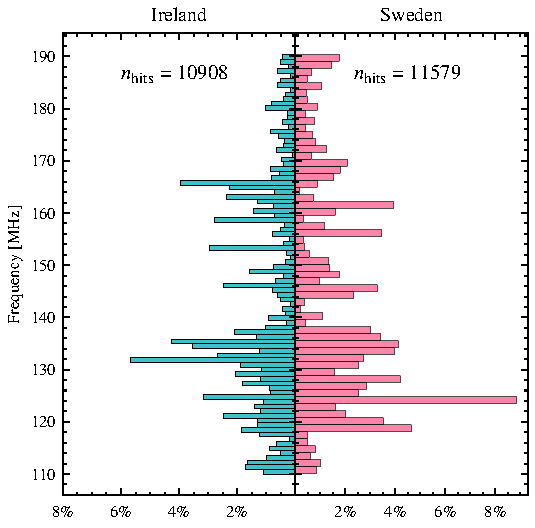
\includegraphics[width = 0.46\textwidth]{figs/hits_comparative_histogram.pdf}}}%
    \qquad
        \subfloat[\centering ]{{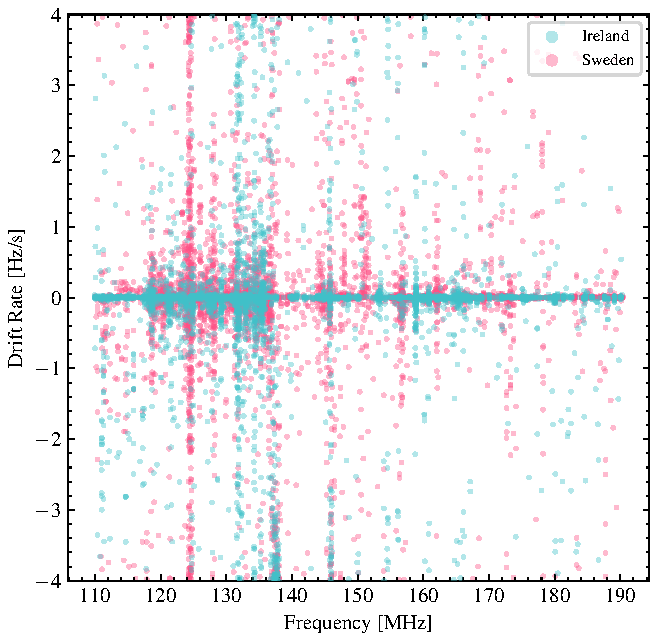
\includegraphics[width=  .46\textwidth]{figs/DR_scatter_plot.pdf}}}%
    \caption{\textit{(a)} Comparison of drifting signals or “hits” detected at both stations seen across the HBA frequency band. Each bin within the data set represents a 1 MHz frequency range and is accompanied by a corresponding percentage indicating its proportion to the overall data set. \textit{(b)} A scatter plot of the drift-rate values against detected frequency. The Irish station is shown in pink and the Swedish station is shown in blue.}%
    \label{fig:hits-histogram}%
\end{figure}

\subsection{Constraints placed by the Survey}

Even though the survey resulted in the non-detection of a narrowband signal it is important to place constraints on the probed parameter space. The required power for a certain  (ETI) transmitter to be detected depends on its directionality and other signal characteristics. 
The transmitter power of an ETI beacon can be measured in terms of the effective isotropic radiated power (EIRP; \citealt{Enriquez2017ApJ}) as,
\begin{equation}
%    {\rm EIRP} = \sigma \times {4 \pi d_\star^2} \frac{\rm SEFD_{\rm HBA}}{\delta{\nu}_{t}} \sqrt{\frac{\delta{\nu}}{n_{p}t_{obs}{\omega}}}  \>\> W/Hz,
    {\rm EIRP} = \sigma \times {4 \pi d_\star^2} \;\frac{{\rm SEFD}}{\delta{\nu_t}}\sqrt{\frac{\delta{\nu}}{n_{p}t_{obs}}}  \>\> \mathrm{W}\;
    \label{Eq:EIRP}
\end{equation}
Here, $\sigma$ is the required S/N, $\delta{\nu}$ is the bandwidth of the received signal, 
$\delta{\nu}_{t}$ is the transmitted bandwidth, $t_{obs}$ is the observing integration time, SEFD is the System Equivalent Flux Density, $n_p$ is the number of polarizations, 
%\omega$ is the duty cycle of the signal, 
and $d_\star$ is the distance between the transmitter and the receiver, i.e., the distance to the star. We considered $\delta{\nu}_{t}$ to be 1\,Hz. For the narrowband signals we consider in our Doppler searches, we assume $\delta{\nu}$ is matched to our spectral resolution and further assume a temporal duty cycle of $100\%$. \ 
%$\omega$ is assumed to be 100\% and $\delta{\nu}$ and $\delta{\nu}_{t}$ is $2.98$~Hz as per our observing specifications.
Figure \ref{fig:EIRP-limits} presents the luminosity limits for the cumulative targets of this survey within the frequency range of $110-190$ MHz. In this figure, the limiting luminosity is compared to notable values of Equivalent Isotropic Radiated Power (EIRP) for various scenarios. These scenarios include a Kardashev I type advanced civilization transmitting at a power level of $10^{17}$ W, an advanced civilization producing planetary radar-level transmissions with a transmitting power of $10^{13}$ W, and a cumulative aircraft radar-type system transmitted across a large solid angle with a power of $10^{10}$ W \citep{Siemion_KEPLER_ApJ}. The figure demonstrates that due to the varying system temperature ($T_{sys}$) across the frequency band, our observations were sensitive to detecting a range of Kardashev I type targets. Specifically, we were able to detect approximately 25\% of the targets at the lower end of the frequency band, increasing to nearly 80\% of the targets at the higher end of the band.

\begin{figure}
    \centering
    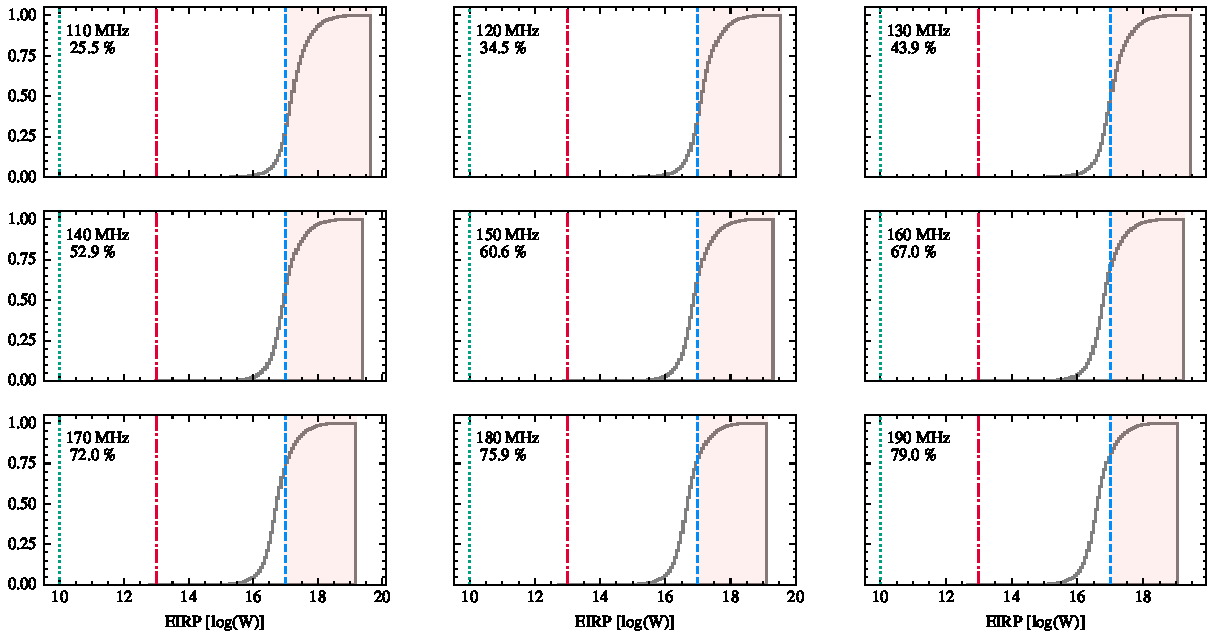
\includegraphics[width = 0.95\textwidth]{figs/EIRP_hist_plot.pdf}
    \caption{Cumulative histogram of EIRP limits of this survey across the HBA band. Reference luminosities for three civilization Kardeshev levels emitting $10^{17}$,$10^{13}$ or $10^{10}$ W are shown in blue, red, and green respectively. The percentage of targets where the station is sensitive to the transmission of $10^{17}$ W is shown, as a function of frequency across the band. At lower frequencies, sensitivity to $10^{17}$ emitters drops off as the $T_{\text{sys}}$ rises. The $\bar T_{\text{sys}}$ varies from 1260 K down to 322 K as frequency is increased across the band. Detailed calculations are presented in Appendix B of \cite{johnson_simultaneous_2023}.}
    \label{fig:EIRP-limits}
\end{figure}

A modified variation of the Drake equation (Eqn.~\ref{eq:modified-drake}; \citealt{Sagan1966, 2022VishalPulsed}) is used to constrain the fraction of narrowband emitting civilizations $(f_c^n)$. 

\begin{equation}
    N =  R_{\text{IP}}f^n_cL
    \label{eq:modified-drake}
\end{equation}

Here  $R_{\text{IP}}$ is defined as the emergence rate $(\text{yr}^{-1})$ of intelligent life in the Milky Way.  \Cref{fig:SETI-constraint} shows the constraint that this survey places on $f_c^n$ when using a Poisson sided upper limit at 95\% confidence which in this case is 2.995 as per \cite{1986_Poission_tables}. This provides the most stringent constraint of $f^n_c$ in this frequency range. \

LOFAR is soon to undergo a staged series of upgrades across all stations in the array. These upgrades at individual stations across Europe will involve the installation of a new Receiver Control Unit (RCU) as described in \cite{LOFAR2}. These RCUs will enable the simultaneous use of both the LBA and HBA in the frequency range of 15 - 240 MHz. This enhancement will allow for a SETI survey across a broader low-frequency band. \ Specifically, at 30 MHz, the FWHM will cover an area of 19.39 deg$^2$, decreasing to 1.73 deg$^2$ at 190 MHz. This will enable follow-up LOFAR surveys to encompass a larger volume of stars and a broader frequency domain. \ 
Additionally during the roll out of the 2.0 upgrade the international stations will be switched into local mode for months at a time. This gives ample opportunity to carry out additional observation campaigns to form the basis of a LOw Frequency pulsar, FRB, and Technosignature Survey (LOFTS). LOFTS will entail a persistent zenith pointings to sweep out sections of the northern hemisphere with a larger $t_{obs}$ and lower $T_{sys}$, greatly improving both the volume and sensitivity of its prior survey. 



\begin{figure}
    \centering
    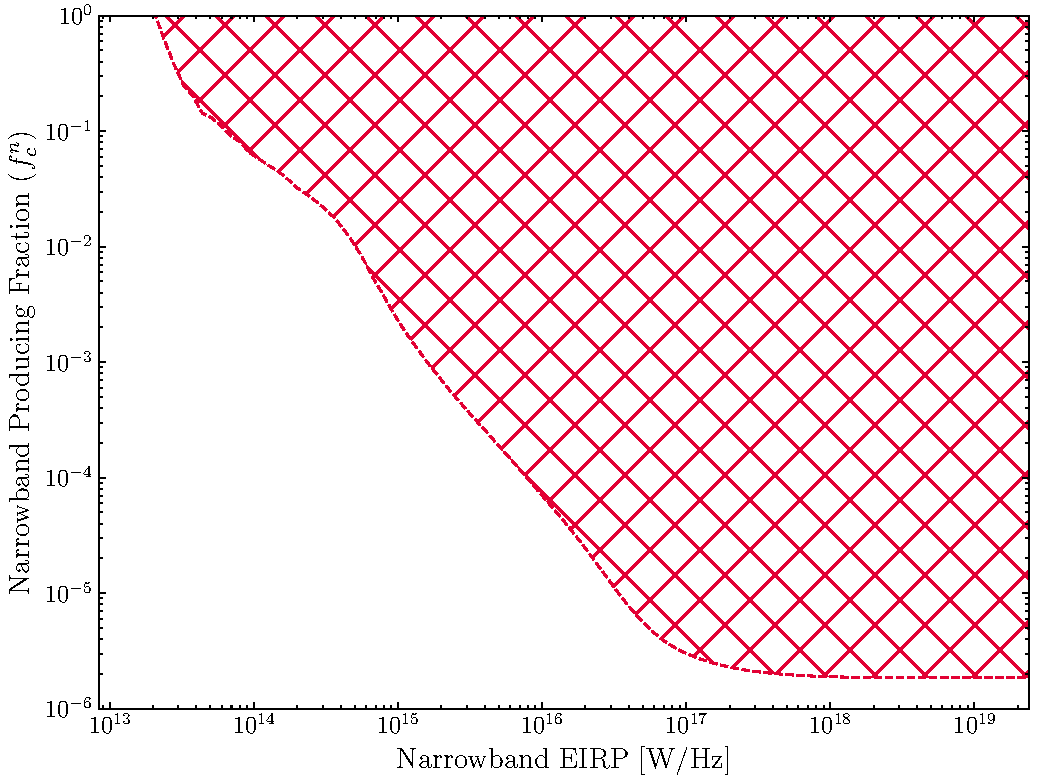
\includegraphics[width = 0.7\textwidth]{figs/narrowband-fraction.pdf}
    \caption{The fraction of stars that produce narrow-band emission ($f^n_c$) against the transmitter power of the total target pool. The hashed region (red) shows the constraints this survey places on a value of $f^n_c$ at 110 - 190 MHz.}
    \label{fig:SETI-constraint}
\end{figure}
